%credits K. Κουνής, I. Στεφανίδου 
%refactoring : K.Draziotis (drazioti@gmail.com
%Licence CC_BY_SA

\documentclass[12pt]{article}
\usepackage{helvet} 
\usepackage{amsmath}
\usepackage{titlesec}
\usepackage{lipsum}
\usepackage{textcomp}
\usepackage{graphicx}
\usepackage{adjustbox}
\graphicspath{{images/}}


\usepackage{listings}
\usepackage{xcolor}

\definecolor{codegreen}{rgb}{0,0.6,0}
\definecolor{codegray}{rgb}{0.5,0.5,0.5}
\definecolor{codepurple}{rgb}{0.58,0,0.82}
\definecolor{backcolour}{rgb}{0.95,0.95,0.92}

\lstdefinestyle{mystyle}{
    backgroundcolor=\color{backcolour},   
    commentstyle=\color{codegreen},
    keywordstyle=\color{magenta},
    numberstyle=\tiny\color{codegray},
    stringstyle=\color{codepurple},
    basicstyle=\ttfamily\footnotesize,
    breakatwhitespace=false,         
    breaklines=true,                 
    captionpos=b,                    
    keepspaces=true,                 
    numbers=left,                    
    numbersep=5pt,                  
    showspaces=false,                
    showstringspaces=false,
    showtabs=false,                  
    tabsize=2
}
\lstset{style=mystyle}

\titleformat{\section}[display]
          {\clearpage\vspace*{50pt}%
          \normalfont\huge\bfseries}%
          {{\Kappa}E{\Phi}A{\Lambda}AIO \thesection}%
          {20pt}%
          {\Huge}%
          [\vspace{40pt}]

\usepackage[algosection,commentsnumbered,ruled,vlined]{algorithm2e}
\usepackage{chemarrow}
\newcommand\aug{\fboxsep=-\fboxrule\!\!\!\fbox{\strut}\!\!\!}
\usepackage{graphicx}
\usepackage{gfsdidot}
\usepackage[LGR,T1]{fontenc}
\usepackage[utf8]{inputenc}
\usepackage[english,greek]{babel} % και για τις δυο γλώσσες
\usepackage{alphabeta}
\usepackage[hidelinks]{hyperref}
\usepackage{hyperref}
\usepackage{makeidx}
\usepackage{enumerate}
\usepackage{float}
\usepackage{enumitem}
\usepackage{systeme}
\usepackage{algorithmic}
\usepackage{comment}
\usepackage{indentfirst}

% TEXT FORMATTING
% set spacing between lines (διάστιχο)
\usepackage{setspace}
\setstretch{1.5}
% package to customize chapters, sections and subsections style
\usepackage{titlesec}
% chapter title appearance format
\titleformat{\chapter}[display]
{\bfseries\huge}{\chaptertitlename\space\thechapter}{16pt}{}
% https://www.sharelatex.com/learN/Sections_and_chapters
\titlespacing{\chapter}{0pc}{1.5ex plus .1ex minus .2ex}{5pc}
% section title appearance format
\titleformat{\section}
{\filright\bfseries\Huge}{Κεφάλαιο \thesection}{12pt}{\\ \vspace{1cm}}[\vspace{2cm}]
% subsection title appearance format
\titleformat{\subsection}
{\bfseries\Large}{\thesubsection}{12pt}{}
% set margins
\usepackage{geometry}
\geometry{left=3cm, right=2cm, top=4cm, bottom=3cm}
\usepackage{graphicx}
% put images in images path
\graphicspath{{images/}}
\usepackage{setspace}

% Caption customization
% use this package to set appearance for captions
\usepackage{caption}
% caption size for figures 10pt
\captionsetup[figure]{font=footnotesize,labelfont=footnotesize}
% caption size for tables 10pt and underlined
\usepackage[normalem]{ulem} % Package for underlining

% use this package to define custom colors
\usepackage{xcolor}

% create colors
\colorlet{punct}{red!60!black}
\definecolor{background}{HTML}{EEEEEE}
\definecolor{delim}{RGB}{20,105,176}
\colorlet{numb}{magenta!60!black}


\usepackage{amsfonts}
\usepackage{amscd}
\usepackage{amssymb}
\newtheorem{algor}{\bf{Algorithm}}[subsection]


\newtheorem{remark}{Remark}[section]

\newtheorem{theorem}{Θεώρημα}[section]
\newtheorem{lemma}[theorem]{Lemma}
% Define definition
\newtheorem{mydef}{Ορισμός}[section]
%\newtheorem{corollary}[theorem]{Corollary}
\newtheorem{definition}[theorem]{Definition}
\newtheorem{proposition}[theorem]{Proposition}
%\theoremstyle{remark}
\newtheorem{example}{Παράδειγμα}[section]
%\newtheorem{remark}[theorem]{Remark}
\numberwithin{equation}{section}

% use this package to show actual code listings
\usepackage{listings}

% change listings name in caption to Απεικόνιση
\renewcommand{\lstlistingname}{Απεικόνιση}

% change listings name in contents page to Κατάλογος απεικονήσεων
\renewcommand\lstlistlistingname{Κατάλογος απεικονίσεων}

% command for congruence/equivalence modulo
\newcommand{\congruence}[3]{\ensuremath{{#1}\equiv {#2}\pmod*{#3}}}
\newcommand{\congr}[2]{\ensuremath{{#1}\left\pmod*{#2}\right}\xspace}
\makeatletter
\let\@@pmod\pmod
\DeclareRobustCommand{\pmod}{\@ifstar\@pmods\@@pmod}
\def\@pmods#1{\mkern4mu({\operator@font mod}\mkern 6mu#1)}
\makeatother

% set custom colorscheme for listings with language=lang1 to make them stand out more
% http://tex.stackexchange.com/questions/83085/how-to-improve-listings-display-of-jsoN-files
\lstdefinelanguage{lang1}{
    basicstyle=\normalfont\ttfamily,
%    numbers=left,
%    numberstyle=\scriptsize,
%    stepnumber=1,
%    numbersep=8pt,
    showstringspaces=false,
    breaklines=true,
    frame=lines,
    backgroundcolor=\color{background},
    literate=
     *{0}{{{\color{numb}0}}}{1}
      {1}{{{\color{numb}1}}}{1}
      {2}{{{\color{numb}2}}}{1}
      {3}{{{\color{numb}3}}}{1}
      {4}{{{\color{numb}4}}}{1}
      {5}{{{\color{numb}5}}}{1}
      {6}{{{\color{numb}6}}}{1}
      {7}{{{\color{numb}7}}}{1}
      {8}{{{\color{numb}8}}}{1}
      {9}{{{\color{numb}9}}}{1}
      {:}{{{\color{punct}{:}}}}{1}
      {,}{{{\color{punct}{,}}}}{1}
      {\{}{{{\color{delim}{\{}}}}{1}
      {\}}{{{\color{delim}{\}}}}}{1}
      {[}{{{\color{delim}{[}}}}{1}
      {]}{{{\color{delim}{]}}}}{1},
}

% create command for blank page
\usepackage{afterpage}
\newcommand\blankpage{%
    \null
    \thispagestyle{empty}%
    \addtocounter{page}{-1}%
    \newpage}
    
\definecolor{maroon}{HTML}{AF3235}
% add clickable hyperlinks
\usepackage{hyperref}
\hypersetup{
    colorlinks,
    citecolor=black,
    filecolor=black,
    linkcolor=black,
    urlcolor=black
}

% use fancy header and footer
\usepackage{fancyhdr}
\usepackage{blindtext} % to quickly get a full document

% Turn on the style
\pagestyle{fancy}

% Clear the header and footer
\fancyhf{}

% Set the right side of the footer to be the page number
\fancyfoot[R]{\thepage}

% set page number appearance to bottom right
\fancypagestyle{plain}{%
    \renewcommand{\headrulewidth}{0pt}
    \fancyhf{}
    \fancyfoot[R]{\thepage}%
}

\newcommand{\HRule}{\rule{\linewidth}{0.5mm}}
\newcommand{\lt}{\latintext}
\renewcommand{\arraystretch}{1.5}

\begin{document}
\begin{titlepage}
\begin{center}


\includegraphics[width=0.3\linewidth]{image.png}
\vspace{1cm}

\textbf{
{\Large \mbox{ΑΡΙΣΤΟΤΕΛΕΙΟ ΠΑΝΕΠΙΣΤΗΜΙΟ ΘΕΣΣΑΛΟΝΙΚΗΣ}}
{\Large ΣΧΟΛΗ ΘΕΤΙΚΩΝ ΕΠΙΣΤΗΜΩΝ} \\
{\Large ΤΗΜΗΜΑ ΠΛΗΡΟΦΟΡΙΚΗΣ}
}
\begin{figure}[h]
\raggedright
\hspace{90pt}
\end{figure}
\centering 

{\Large \textbf{ Ανάλυση αλγορίθμων παραγοντοποίησης}}

\vspace{1cm}
{\large \textbf{Μεταπτυχιακή Διπλωματική εργασία \\ Καλαθάς Εμμανουήλ}  \par}

{\large\textbf{Επιβλέπων καθηγητής: Δρ. Δραζιώτης Κωνσταντίνος} \par}
\clearpage
\vfill



\begin{center}
    
\includegraphics[width=0.3\linewidth]{image.png}
\end{center}

\vspace{1cm}
\lt{
\textbf{
{\Large {ARISTOTLE UNIVERSITY OF THESSALONIKI}
{\Large FACULTY OF SCIENCES} \\
{\Large SCHOOL OF INFORMATICS}
}}}
\begin{figure}[h]
\raggedright
\hspace{90pt}
\end{figure}
\centering 

{\Large \textbf{\lt{Analysis of factorization algorithms}}}

\begin{doublespacing}
\vspace{1cm}
{\large 
\textbf{\lt{Post Graduate Thesis \\ Kalathas Emmanouil}} \par}

{\large
\textbf{\lt{Supervisor: Dr. Draziotis Konstantinos}} \par}
\clearpage
\vfill
\end{doublespacing}
\end{center}

\includegraphics[width=0.2\linewidth]{image.png}
\textbf{\lt{Copyright ©All rights reserved Καλαθάς Εμμανουήλ, 2023.}}
\vspace{0.5cm} \\
\small{Με πλήρη επίγνωση των συνεπειών του νόμου περί πνευματικών δικαιωμάτων,
δηλώνω ρητά ότι η παρούσα πτυχιακή εργασία, καθώς και τα ηλεκτρονικά αρχεία και πηγαίοι κώδικες που αναπτύχθηκαν ή τροποποιήθηκαν στο πλαίσιο
αυτής της εργασίας, αποτελεί αποκλειστικά προϊόν προσωπικής μου εργασίας,
δεν προσβάλλει κάθε μορφής δικαιώματα διανοητικής ιδιοκτησίας, προσωπικότητας και προσωπικών δεδομένων τρίτων, δεν περιέχει έργα/εισφορές τρίτων
για τα οποία απαιτείται άδεια των δημιουργών/δικαιούχων και δεν είναι προϊόν
μερικής ή ολικής αντιγραφής, οι πηγές δε που χρησιμοποιήθηκαν περιορίζονται
στις βιβλιογραφικές αναφορές και μόνον και πληρούν τους κανόνες της επιστημονικής παράθεσης. Τα σημεία όπου έχω χρησιμοποιήσει ιδέες, κείμενο, αρχεία
ή/και πηγές άλλων συγγραφέων, αναφέρονται ευδιάκριτα στο κείμενο με την
κατάλληλη παραπομπή και η σχετική αναφορά περιλαμβάνεται στο τμήμα των
βιβλιογραφικών αναφορών με πλήρη περιγραφή. Αναλαμβάνω πλήρως, ατομικά
και προσωπικά, όλες τις νομικές και διοικητικές συνέπειες που δύναται να προκύψουν στην περίπτωση κατά την οποία αποδειχθεί, διαχρονικά, ότι η εργασία
αυτή ή τμήμα της δεν μου ανήκει διότι είναι προϊόν λογοκλοπής. 
\vspace{0.5cm} \\
Το περιεχόμενο αυτής της εργασίας δεν απηχεί απαραίτητα τις απόψεις του
Τμήματος, του Επιβλέποντα, ή της επιτροπής που την ενέκρινε.}
\vspace{0.7cm} \\
\begin{doublespacing}
\textbf{Υπεύθυνη Δήλωση} \\
\textbf{Υπογραφή .........................................................} \\
\textbf{Καλαθάς Εμμανουήλ}
\end{doublespacing}

\blankpage
\end{titlepage}
\newpage

% insert table of contents
\tableofcontents

\clearpage

% leave blank page before main part
\blankpage

\begin{center}
    {\textbf{\Large{Περίληψη}}}
\end{center}
\vspace{0.5cm}

Η εργασία αυτή αναλύει και επεξηγεί διάφορους αλγόριθμους παραγοντοποίησης ακέραιων αριθμών, εμπεριέχοντας και την υλοποίηση τους στη γλώσσα Python. Για την ταχύτερη εκτέλεση του προγράμματος χρησιμοποιήθηκε η Cython, ένας στατικός μεταγλωττιστής της Python, καθώς και η βιβλιοθήκη gmpy2 για την υποστήριξη μεγάλων και πολλαπλής ακρίβειας ακεραίων καθώς και συμβατότητα με την Cython.  Αρχικά, γίνεται μια αναφορά στο σύστημα RSA και την σημασία που έχει η παραγοντοποίηση μεγάλων ακεραίων για την ασφάλεια αυτού αλλά και της επικοινωνίας μέσω μη ασφαλών μέσων όπως το διαδίκτυο. Στη συνέχεια, αναλύονται βασικοί αλγόριθμοι  όπως αυτός της δοκιμαστικής διαίρεσης, της μεθόδου \lt{Fermat}, του αλγορίθμου Pollard Rho καθώς και του Quadratic Sieve που αποτελεί τον ταχύτερο αλγόριθμο παραγοντοποίησης για αριθμούς με κάτω από 100 δεκαδικά ψηφία.

Ο κώδικας μπορεί να βρεθεί \href{https://github.com/inco0/Factorization}{εδώ}.

\newpage

\begin{center}
    {\textbf{\Large{Summary}}}
\end{center}
\vspace{0.5cm}


This paper analyzes and explains various algorithms for integer factorization, including their implementation in Python. For the purpose of faster excution time, the Cython module, a statically typed compiler for Python, was used along with the gmpy2 library in order to support big and multiple precision integers as well as compatibility for Cython. Initially, the RSA system is briefly mentioned along with the importance of factoring large integers for its security as well as for communicating via insecure means such as the internet. Next, basic algorithms such as trial division, Fermat's method, and Pollard Rho are analyzed, as well as the Quadratic Sieve, which is the fastest factorization algorithm for numbers with around 100 decimal digits.

The code can be found here \href{https://github.com/inco0/Factorization}{εδώ}.

\newpage

\section{Εισαγωγή}

\subsection{Κρυπτοσύστημα \lt{RSA}}
 Το 1978 οι \lt{Ron Rivest, Adi Shamir, Leonard Adleman} δημοσίευσαν ένα άρθρο \cite{rsa78} στο οποίο εισήγαγαν την έννοια ενός κρυπτοσυστήματος δημοσίου κλειδιού. Σήμερα, η ασφάλεια μεταφοράς δεδομένων μέσω του διαδικτύου βασίζεται σε μεγάλο βαθμό στο \lt{RSA}. Αποτελείται από τέσσερα βήματα, την παραγωγή κλειδιών, την μεταφορά τους, την κρυπτογράφηση και αποκρυπτογράφηση μηνυμάτων.

\begin{mydef}[RSA]
    Ως κρυπτοσύστημα RSA ορίζεται ένα σύνολο πέντε στοιχείων \{M,C,K,E,D\}, όπου:
    \begin{itemize}
        \item M: Ο χώρος των μηνυμάτων
        \item C: Ο χώρος των κρυπτογραφημένων μηνυμάτων
        \item K: Ο χώρος των κλειδιών
        \item E: Οι συναρτήσεις κρυπτογράφησης
        \item D: Οι συναρτήσεις αποκρυπτογράφησης
    \end{itemize}
\end{mydef}
 
\subsubsection{Παραγωγή κλειδιών}
\begin{enumerate}
\item Επιλέγουμε αρχικά δύο πρώτους \lt{p, q} \cite{rsa78}. 
\begin{itemize}
    \item Οι δύο αυτοί αριθμοί είναι καθοριστικοί για την ασφάλεια του συστήματος και πρέπει να έχουν κάποιες συγκεκριμένες ιδιότητες.
    \item Να είναι επιλεγμένοι τυχαία.
    \item Να μην είναι γνωστοί σε άλλους.
    \item Να είναι επαρκώς μεγάλοι - η τάξη μεγέθους εξαρτάται από το σύστημα και συνήθως είναι 2048 bit και παραπάνω.
    \item Να μην είναι κοντά μεταξύ τους ώστε να μην είναι ευάλωτοι στην παραγοντοποίηση με τη μέθοδο του \lt{Fermat}.
\end{itemize}

\item Υπολογίζουμε $N = pq$.
\begin{itemize}
    \item Το $N$ χρησιμοποιείται σαν \lt{modulo}, τόσο στο δημόσιο όσο και στο ιδιωτικό κλειδί.
    \item Το $N$ δημοσιεύεται σαν μέρος του δημόσιου κλειδιού.
\end{itemize}

\begin{mydef}[Συνάρτηση \lt{Carmichael} \cite{pomerance1991carmichael}]
Η συνάρτηση \lt{Carmichael} $λ(N)$ ενός θετικού ακέραιου αριθμού είναι ο μικρότερος θετικός ακέραιος $m$ έτσι ώστε για κάθε ακέραιο α σχετικά πρώτο με το $N$ να ισχύει:
\begin{align}
    \congruence{a^m}{1}{n} \nonumber
\end{align}
\end{mydef}

\begin{mydef}[Συνάρτηση \lt{Euler} \cite{euler1879}]
Για κάθε θετικό ακέραιο $N$, το $\phi(N)$ έχει σαν τιμή, το πλήθος των φυσικών αριθμών μικρότερων του $N$ οι οποίοι είναι σχετικά πρώτοι με αυτό.
\end{mydef}

\item Υπολογίζουμε το $λ(N)$. Επειδή $N=pq, λ(N)=lcm(λ(p), λ(q))$, και από τον ορισμό των δύο προηγούμενων συναρτήσεων ισχύει ότι $λ(p)=\phi(p)=p-1$ και ομοίως $λ(q)=\phi(q)=q-1$, άρα $λ(N)=lcm(p-1, q-1)$.
\begin{itemize}
    \item Η συνάρτηση \lt{lcm} είναι το ελάχιστο κοινό πολλαπλάσιο δύο τιμών.
    \item Η \lt{lcm} μπορεί να υπολογιστεί με τον αλγόριθμο του Ευκλείδη.
\end{itemize}

\item Επιλέγουμε έναν ακέραιο $e$ τέτοιον ώστε $2<e<λ(N)$ και $gcd(e, λ(N))=1$, να είναι δηλαδή σχετικά πρώτος με το $λ(N)$.
\begin{itemize}
    \item Μικρότερες τιμές του $e$ οδηγούν σε πιο αποδοτική κρυπτογράφηση αλλά είναι ευάλωτες σε συγκεκριμένες επιθέσεις\cite{boneh1999twenty}. Μια κοινή τιμή του $e$ είναι η $2^{16}+1=65537$ λόγω της ταχύτητας που προσφέρει στην κρυπτογράφηση.
    \item Το $e$ δημοσιεύεται μαζί με το δημόσιο κλειδί.
\end{itemize}

\item Υπολογίζουμε το:
\begin{align}
    \label{d-calc}
    \congruence{d}{e^{-1}}{λ(N)}
\end{align}
\begin{itemize}
    \item Το $d$ μπορεί να υπολογιστεί από τον εκτεταμένο αλγόριθμο του Ευκλείδη, αφού τα $e,λ(N)$ είναι σχετικά πρώτοι μεταξύ τους.
    \item Το $d$ είναι μέρος του ιδιωτικού κλειδιού.
\end{itemize}
\end{enumerate}

Επομένως, το δημόσιο κλειδί αποτελείται από το \lt{modulo N} και το δημόσιο εκθέτη \lt{e} και το ιδιωτικό κλειδί από τον εκθέτη \lt{d} και τα \lt{p,q,}$λ(N),\phi(N)$.

\begin{theorem}
    Εάν το N είναι το γινόμενο δύο πρώτων p και q, τότε μπορούμε να παραγοντοποιήσουμε το N σε πολυωνυμικό χρόνο, γνωρίζοντας το N και το $\phi(N)$. 
\end{theorem}

\textbf{Απόδειξη.} Έχουμε ότι $\phi(N)=(p-1)(q-1)=N-(p+q)+1$ και $N=pq$. Τότε, $N+1-\phi(N)=p+q=p+N/p$ ή $p-(N+1-\phi(N))+N/p=0 \iff p^2-(N+1-\phi(N))p+n=0$.
Λύνοντας την παραπάνω εξίσωση, μπορούμε να αποκτήσουμε τα p και q.\\

 Το παραπάνω θεώρημα εξηγεί γιατί τα $λ(N),\phi(N)$ πρέπει να κρατηθούν κρυφά για να παραμείνει ασφαλές το RSA.

\subsubsection{Κρυπτογράφηση}
Έστω, ότι ο Γιάννης θέλει να επικοινωνήσει με την Αλίκη, τότε αν συμφωνήσουν να χρησιμοποιήσουν το \lt{RSA} ο Γιάννης πρέπει να αποκτήσει το δημόσιο κλειδί της Αλίκης μέσα από ένα αξιόπιστο μέσο, χωρίς δηλαδή να μπορεί κάποιος να αλλάξει τα περιεχόμενα του μηνύματος χωρίς αυτό να γίνει αντιληπτό αλλιώς η επικοινωνία τους είναι ευάλωτη σε μια επίθεση \lt{man in the middle}\cite{maurer1994calculus}. \\
Αρχικά, μετατρέπει το μήνυμα του σε έναν ακέραιο m με $0\leq{m}<n$ και υπολογίζει το κρυπτογραφημένο μήνυμα \lt{c}, χρησιμοποιώντας το δημόσιο κλειδί της Αλίκης \lt{e}, που αντιστοιχεί στο: 
\begin{align}
    \congruence{c}{m^e}{n} \nonumber
\end{align}

\subsubsection{Αποκρυπτογράφηση}
Για να αποκρυπτογραφήσει το μήνυμα η Αλίκη χρησιμοποιεί το ιδιωτικό της κλειδί \lt{d}, υπολογίζοντας:
\begin{align}
    c^d \equiv \congruence{(m^e)^d}{m}{n} \nonumber
\end{align}

Πρέπει να σημειωθεί ότι το μήνυμα, δεν μεταδίδεται όπως είναι αλλά χρησιμοποιείται ένα σχήμα συμπλήρωσης (padding scheme) το οποίο γνωρίζουν τόσο ο παραλήπτης όσο και ο αποδέκτης. Αυτό το βήμα είναι απαραίτητο για την αποφυγή επιθέσεων γνωστού κειμένου \cite{coron2000new}.

\begin{example}
\end{example}
Επιλέγουμε δύο πρώτους $p=11$ και $q=13$ και υπολογίζουμε το $N=143$, το $\phi(N)=120$ και το $λ(N)=lcm(10,12)=60$. Επιλέγουμε έναν ακέραιο $e$ έτσι ώστε $2<ε<λ(N)$ και $gcd(e,λ(N))=1$. Έστω ότι $e=7$, υπολογίζουμε το $\congruence{d}{e^{-1}}{λ(N)}$ που μας δίνει $d=43$, άρα έχουμε το ιδιωτικό κλειδί $(p=11, q=13, d=43$ και το δημόσιο κλειδί $(n=143, e=13)$. 

Για να κρυπτογραφήσουμε το μήνυμα $m=47$ υπολογίζουμε την τιμή του $c=m^e= \congruence{47^{43}}{5}{143}$. 

Για να αποκρυπτογραφήσουμε το c, υπολογίζουμε το $m={c^d}=(m^e)^d= \congruence{(47^{13})^{43}}{47}{143}$

\subsection{Επιθέσεις στο \lt{RSA}}
Η ασφάλεια του RSA βασίζεται εξ' ολοκλήρου στην δυσκολία παραγοντοποίησης μεγάλων ακεραίων. Αν από το Ν μπορούμε να βρούμε τα p και q, τότε μπορεί εύκολα να υπολογιστεί και το $λ(N)$ και κατά συνέπεια το d από την \ref{d-calc}.

Αν κάποιος δεν γνωρίζει τον εκθέτη αποκρυπτογράφησης, τότε το να αντιστραφεί η συνάρτηση κρυπτογράφησης είναι ιδιαίτερα δύσκολο και γνωστό ως πρόβλημα RSA. Μπορούμε άρα να πούμε ότι το να λύσει κάποιος το RSA είναι τουλάχιστον όσο δύσκολο όσο η παραγοντοποίηση.

\subsubsection{Επίθεση \lt{Wiener}}
Όπως προαναφέρθηκε, η τιμή του εκθέτη αποκρυπτογράφησης επηρεάζει την ταχύτητα αυτής. Ωστόσο, η επιλογή μικρών τιμών υπό κάποιες συνθήκες ελοχεύει κινδύνους όπως απέδειξε ο Wiener \cite{wiener1990cryptanalysis} το 1990, ο οποίος με τη χρήση συνεχών κλασμάτων κατάφερε να ανακτήσει τον εκθέτη αποκρυπτογράφησης.

\begin{theorem}[Wiener] Υπάρχει αλγόριθμος πολυωνυμικού χρόνου, ο οποίος παραγοντοποιεί το N δεδομένου το e, αν $e<)$ και $N=pq$, όπου p και q είναι άγνωστοι πρώτοι με $q<p<2p$ και υπάρχει ακέραιος $d<\sqrt[4]{N}/3$ που ικανοποιεί τη σχέση $\congruence{ed}{1}{k}$.\\
\end{theorem}

\textbf{Απόδειξη.} Αφού ισχύει $\congruence{ed}{1}{\phi(N)}$, τότε υπάρχει ακέραιος k τέτοιος ώστε $ed-k\phi(N)=1$. Διαιρώντας με το $d\phi(N)$ παίρνουμε:

\begin{align}
    \left\lvert \frac{e}{\phi(N)} - \frac{k}{d} \right\rvert = \frac{1}{d\phi(N)}.
\end{align}

Αν θεωρήσουμε ότι το Ν είναι μία προσέγγιση του $\phi(N)$ και επειδή έχουμε $q < p < 2q$ και $N=pq$, τότε $q < \sqrt{N}$ και $0 < Ν - \phi(N) = p + q - 1 < 3q -1 < 3\sqrt{N}$ και $ed = 1 + k\phi(N)$. Αντικαθιστώντας στην (1.2) έχουμε:

\begin{align}
    \left\lvert \frac{e}{N} - \frac{k}{d} \right\rvert = \left\lvert \frac{ed-kN}{dN} \right\rvert = 
    \left\lvert \frac{1-k(N-\phi(N))}{dN} \right\rvert.
\end{align}

Έχουμε ότι $0 < N - \phi(N) < 3 \sqrt{N}$, άρα:

\begin{align}
    \left\lvert \frac{e}{N} - \frac{k}{d} \right\rvert \leq \left\lvert \frac{3k\sqrt{N}}{dN} \right\rvert = \frac{3k}{d\sqrt{N}}
\end{align}

Ισχύει ότι, $k\phi(N) = ed - 1 < ed$ και $e < \phi(N)$. Από πριν έχουμε $k < d < \sqrt[4]{N}/3$. Αντικαθιστώντας στην (1.4) έχουμε:

\begin{align}
    \left\lvert \frac{e}{N} - \frac{k}{d} \right\rvert \leq \frac{1}{d\sqrt[4]{N}} < \frac{1}{2d^2}.
\end{align}

\begin{theorem}[Εύρεση συγκλινόντων συνεχών κλασμάτων \cite{niven1991introduction}]
    Έστω ότι Α και Β ακέραιοι με $\gcd(A,B)=1$ και 
    \begin{align}
        \left \lvert \frac{A}{B} - x \right \rvert < \frac{1}{2B^2},
    \end{align}
    τότε υπάρχει $k>0$ τέτοιο ώστε το κλάσμα $Α_k$ και $B_k$ να είναι ένας από τους συγκλίνοντες στο x. 
\end{theorem}

Γνωρίζοντας ότι οι $e$ και $N$ είναι μεταξύ τους πρώτοι και χρησιμοποιώντας το παραπάνω θεώρημα στην (1.5),
μπορούμε σε πολυωνυμικό χρόνο να υπολογίσουμε τους συγκλίνοντες του κλάσματος $\frac{e}{N}$ και άρα το d.

\clearpage

\section{Βασικοί αλγόριθμοι παραγοντοποίησης}
\subsection{Δοκιμαστική διαίρεση}
Ο πιο απλός αλγόριθμός παραγοντοποίησης, η δοκιμαστική διαίρεση, παραγοντοποιεί έναν ακέραιο Ν διαιρώντας τον διαδοχικά με πρώτους αριθμούς. Κάθε πρώτος που διαιρεί το Ν, έστω \lt{p}, αποθηκεύεται και αφαιρείται από το Ν όσες φορές η διαίρεση τους είναι ακέραια. Αυτό συνεχίζεται, μέχρι ο επόμενος πρώτος αριθμός να γίνει μεγαλύτερος από την ρίζα του εναπομείναντα Ν. Στη συνέχεια, βρίσκει τον τελευταίο διαιρέτη και σε περίπτωση που ο Ν είναι πρώτος, τότε τυπώνει ένα αντίστοιχο μήνυμα.

Στον συγκεκριμένο αλγόριθμο θεωρούμε ότι έχουμε τους πρώτους αριθμούς - βρίσκοντας τους για παράδειγμα με το κόσκινο του Ερατοσθένη - και ελέγχουμε μόνο αυτούς  μέχρι την ρίζα του Ν. Ο ίδιος αλγόριθμος λειτουργεί, αν και πιο αργά, αυξάνοντας το p ανά δύο ελέγχοντας τους περιττούς αριθμούς μετά το 3. Λόγω της ιδιότητας της να ελέγχει πρώτα για διαιρέτες με μικρές τιμές, η δοκιμαστική διαίρεση είναι μία καλή επιλογή όταν παραγοντοποιούμε ομαλούς αριθμούς, που έχουν δηλαδή μόνο μικρούς διαιρέτες.

\vspace{0.5cm}
\begin{algorithm}[H]
\lt{
\SetAlgoLined
\KwIn{Ένας ακέραιος $N > 1$}
$m \gets N$\;
$p \gets 2$\;
\While{$p \leq \sqrt{m}$}{
    \If{$(m \bmod p) = 0$}{
        \quad\quad  Print $p$ divides $N$\\
        \quad\quad $m \gets m / p$\
    }
    \Else{
        \quad\quad $p \gets$ the next prime after $p$\
    }
}
\If{$m = N$}{
    \quad\quad Print $N$ is prime\
}
\ElseIf{$m > 1$}{
    \quad\quad Print $m$ divides $N$\
}
\KwOut{Οι πρώτοι παράγοντες του $N$}
\caption{Δοκιμαστική διαίρεση}
}
\end{algorithm}

\subsection{Παραγοντοποίηση \lt{Fermat}}
Η παραγοντοποίηση Fermat, επονομαζόμενη από τον Pierre de Fermat βασίζεται στην αναπαράσταση μονών ακεραίων σαν διαφορά δύο τετραγώνων:
\begin{align}
    N = a^2 - b^2 \nonumber
\end{align}
Η διαφορά αυτή παραγοντοποιείται ως $(a+b)(a-b)$, αν κανένας από τους δύο παράγοντες δεν αντιστοιχεί στο ένα όπου και έχουμε μία τετριμμένη λύση. Ο αλγόριθμος για την παραγοντοποίηση Fermat είναι ο ακόλουθος:

\vspace{0.5cm}
\begin{algorithm}[H]
\SetAlgoLined
\KwIn{Ένας περιττός θετικός ακέραιος $N$ που θα παραγοντοποιηθεί}
$x \gets \sqrt{N}$\;
$t \gets 2x + 1$\;
$r \gets x^2 - N$\;
\While{$r$ is not a square}{
    \quad\quad $r \gets r + t$\;
    \quad\quad $t \gets t + 2$\;
}
$x \gets (t - 1) / 2$\;
$y \gets \sqrt{r}$\;
\KwOut{Οι παράγοντεςt του Ν είναι οι $x - y$ και $x + y$}
\caption{Παραγοντοποίηση με τη μέθοδο του Fermat}
\end{algorithm}
\vspace{0.5cm}

Η μεταβλητή r λαμβάνει τις τιμές $x^2 - N, (x+1)^2 - N, (x+2)^2 - N,$ μέχρι το αποτέλεσμα αυτό να είναι τετράγωνο. Αυτό γίνεται με την πρόσθεση μονών αριθμών της μεταβλητής t που κάθε φορά αυξάνεται κατά δύο για τη δημιουργία τετραγώνων. Όταν ο while βρόχος τερματίσει θα έχουμε μία εξίσωση της μορφής $r = (x+k)^2 - N \iff N = a^2 - r = a^2 - y^2$, άρα ως διαφορά δύο τετραγώνων θα έχει παραγοντοποιηθεί και το Ν. 

\begin{example}[Παραγοντοποίηση με τη μέθοδο Fermat]
\end{example}
Έστω ότι θέλουμε να παραγοντοποιήσουμε τον αριθμό $Ν=527$. Οι τιμές των μεταβλητών κατά τη διάρκεια της εκτέλεσης του αλγορίθμου φαίνονται στον παρακάτω πίνακα. \\
\begin{center}
    \begin{tabular}{|c|c|c|c|}
        \hline
        $x$ & $t=2x+1$ & $x^2$ & $r=x^2-N$ \\
        \hline
        $22$ & $45$ & $484$ & $-43$ \\
        \hline
        $23$ & $47$ & $529$ & $2$ \\
        \hline
        $24$ & $49$ & $576$ & $49=7^2$ \\
        \hline
    \end{tabular}
\end{center}
\vspace{0.5cm}
Η τελευταία γραμμή μας δίνει την παραγοντοποίηση $527=24^2-7^2=(24-7)(24+7)=17*31$

\begin{theorem}[Πολυπλοκότητα του αλγορίθμου παραγοντοποίησης του Fermat \cite{wagstaff2013joy}]
Έστω ο μοναδικός περιττός σύνθετος θετικός αριθμός $N = ab$, όπου $a$ είναι ο μεγαλύτερος διαιρέτης του $N$ που είναι $\leq \sqrt{N}$. Έστω $k = a/\sqrt{N}$, έτσι ώστε $0 < k \leq 1$. Τότε οι οδηγίες του βρόχου while στον αλγόριθμο παραγοντοποίησης του Fermat εκτελούνται $1 + (1 - k)^2 \sqrt{N}/(2k)$ φορές.
\end{theorem}

\textbf{Απόδειξη}
Αν $a = b$, τότε το $N$ είναι τετράγωνο, $k = 1$ και ο βρόχος while τερματίζει μετά την πρώτη επανάληψη. Σε κάθε περίπτωση, όταν ο αλγόριθμος τελειώσει, ισχύει $x - y = a$ και $x + y = b$, δηλαδή $x = (a + b)/2$ και $y = (b - a)/2$. Τη στιγμή αυτή, έχουμε $x = (t - 1)/2$, άρα $t = 1 + a + b = 1 + a + N/a$. Η μεταβλητή $t$ αυξάνεται κατά 2 σε κάθε επανάληψη, ξεκινά από το πρώτο περιττό αριθμό $> \sqrt{N}$ και σταματά στο $1 + a + N/a$. Συνεπώς, ο βρόχος while εκτελείται:

\begin{align}
    1 + \frac{1}{2} \left ( \left ( a + \frac{N}{a} \right ) - 2 \sqrt{N} \right ) = 1 + \frac{{(\sqrt{N} - a)}^2}{2a} = 1 + \frac{{(1-k)}^2}{2k}\sqrt{N} \nonumber
\end{align}

\subsection{Παραγοντοποίηση \lt{Hart}}
Ο William Hart \cite{hart2012one} εφηύρε μία παραλλαγή της μεθόδου του Fermat, που δουλεύει ως εξής. Αρχικά ελέγχει αν ο N είναι τετράγωνο και αν δεν είναι εκτελεί δοκιμαστική διαίρεση όπως ο αλγόριθμός 2.1 αλλά σταματάει μόλις το p φτάσει την τιμή $N^{1/3}$. Αν δεν έχει τελειώσει η παραγοντοποίηση, ακολουθούνται τα επόμενα βήματα:

Για $i =1,2,3,...,$ ελέγχει αν η τιμή ${(\lceil \sqrt{Ni} \rceil)}^2 mod N$ είναι τετράγωνο. Αν αυτός ο αριθμός ισούται με το $t^2$, τότε ο $gcd(\lceil \sqrt{Ni} - t, N)$ είναι παράγοντας του Ν.

\vspace{0.5cm}
\begin{algorithm}[H]
\lt{
\SetAlgoLined
\KwIn{Ένας ακέραιος Ν και ένα όριο L}
\For{$i\leftarrow 1$ \KwTo $L$}{
  $s\leftarrow \lceil \sqrt{Ni}\rceil $\;
  $m\leftarrow s^2\bmod N$\;
  \If{$m$ is a square}{
    \textbf{break}\;
  }
}
$t\leftarrow \sqrt{m}$\;
\KwOut{Η τιμή του gcd(s - t, N) είναι παράγοντας του Ν}
\caption{Παραγοντοποίηση του Hart}
}
\end{algorithm}

\subsection{Παραγοντοποίηση \lt{Pollard Rho}}
Την δεκαετία του εβδομήντα ο John Pollard \cite{monte-carlo-factorization} σκέφτηκε δύο μεθόδους γρηγορότερες από την δοκιμαστική διαίρεση, για την εύρεση μικρών πρώτων παραγόντων. 

Έστω Ν ο αριθμός που θέλουμε να παραγοντοποιήσουμε και p ένας άγνωστος πρώτος παράγοντας του Ν. Επιλέγουμε μία τυχαία συνάρτηση $f$ από το σύνολο s={0,1,..,N-1} στον εαυτό της, ξεκινώντας από έναν τυχαίο αρχικό αριθμό n στο σύνολο αυτό επαναλαμβάνοντας την $f$ ως εξής:
\begin{align}
    s, f(s), f(f(s)), f(f(f(s))),.. \nonumber
\end{align}

Εφόσον η $f$ παίρνει τιμές σε ένα πεπερασμένο σύνολο τιμών και λόγω του παράδοξου των γενεθλίων, περιμένουμε η ακολουθία να έχει επαναλαμβανόμενες τιμές, συγκεκριμένα, μετά από περίπου $\sqrt{p}$ επαναλήψεις και ύστερα να γίνει κυκλική. Εάν δύο αριθμοί $k, m$ είναι τιμές της $f$ με $\congruence{k}{m}{p}$, τότε είναι πιθανό ότι $gcd(k-m, N)=p$ αφού ο $p$ διαιρεί το $k-m$ και τον Ν και επιπλέον κανένας άλλος πρώτος παράγοντας του Ν δεν διαιρεί το $k-m$. 

Έστω ότι ορίζουμε τα $s_i$ ως $s_0=s, s_i=f(s_{i-1}), i>0$. Αν $\congruence{s_i}{s_j}{p}, $ τότε το $p$ διαιρεί το $s_i-s_j$ και επίσης το $gcd(s_i-s_j, N)$. Ωστόσο, δεν μπορούμε να υπολογίσουμε το μέγιστο κοινό διαιρέτη για όλα τα ζεύγη $i,j<\sqrt{p}$ διότι η πολυπλοκότητα του αλγορίθμου θα αναγόταν σε αυτή της δοκιμαστικής διαίρεσης.

Για να λύσουμε αυτό το πρόβλημα βρίσκουμε δύο τιμές της συνάρτησης $f$, $s_m$ και $s_{2m}$ σε μία επανάληψη με την μία να έχει την διπλάσια τιμή της άλλης, υπολογίζοντας το $gcd(s_{2m}-s_m, N)$ ελπίζοντας να βρούμε το $p$. 

\newpage

Στη συνέχεια φαίνεται ο ψευδοκώδικας για τον αλγόριθμο Pollard Rho:
 
\vspace{0.5cm}
\begin{algorithm}[H]
\SetAlgoLined
\KwIn{Ένας σύνθετος ακέραιος $N$ που θα παραγοντοποιηθεί.}
\KwOut{Ένας παράγοντας $g$ του $N$, αλλιώς αποτυχία."}
Pick a random $b$ in $1 \leq b \leq N-3$; \\
Pick a random $s$ in $0 \leq s \leq N-1$; \\
$A \leftarrow s$; \\
$B \leftarrow s$; \\
$g \leftarrow 1$; \\ 
Define a function $f(x) \leftarrow (x^2 + b) \mod N$; \\
\While{$(g = 1)$}{ 
$A \leftarrow f(A)$; \\
$B \leftarrow f(f(B))$; \\
$g \leftarrow \gcd(A-B,N)$; 
}
\If{$(g<N)$}{
Print $g$ "is a proper factor of" $N$;
}
\Else{
Either give up or try again with new $s$ and/or $b$;
}
\caption{Pollard Rho αλγόριθμος για την παραγοντοποίηση ενός σύνθετου ακεραίου $N$.}
\end{algorithm}
\newpage

\begin{example}
\end{example} 
    Παραγοντοποίηση του $N = 25279$ με τη μέθοδο του Pollard Rho, όπου $s = b = 1$.
Οι πρώτες 13 επαναλήψεις $\bmod N$ είναι $s_0=1, s_1=2, s_2=5, s_3=26, s_4=677,
s_5=3308, s_6 = 22337, s_7=9947, s_8=804, s_9=14442, s_{10}=19615, s_{11}=1846, s_{12}=20331$. Έχουμε $gcd(s_{12}-s_6, N) = gcd(20331-22337, 25279) = 17$. Οι τιμές του $s_i \bmod 17$ φαίνονται στο παρακάτω σχήμα. Η μορφή του σχήματος είναι η αιτία για το όνομα του αλγορίθμου.

\begin{figure}[H]
    \centering
    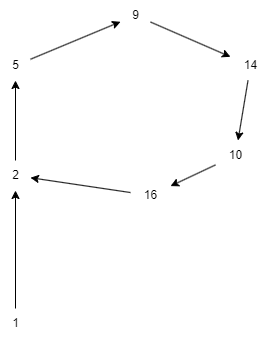
\includegraphics[width=0.4\linewidth]{pollardrho.png}
    \caption{Pollard Rho modulo 17}
\end{figure}

\clearpage

\section{Αλγόριθμος \lt{Quadratic Sieve}}

\subsection{Εισαγωγή}
Όλοι οι αλγόριθμοι που έχουμε εξετάσει μέχρι τώρα είναι εκθετικής πολυπλοκότητας με τον χρόνο εκτέλεσης τους να ανεβαίνει εκθετικά σε σχέση με την είσοδο - τον αριθμό που έχουμε να παραγοντοποιήσουμε. Το 1982 ο Carl Pomerance \cite{lenstra1982analysis} δημοσίευσε τον Quadratic Sieve που βασίζεται σε μεγάλο βαθμό στη μέθοδο συνεχών κλασμάτων των Morrison και Brillhart \cite{morrison1975method} και ανήκει σε μία κατηγορία αλγορίθμων υποεκθετικής πολυπλοκότητας μαζί με τον Number Field Sieve και την μέθοδο ελλειπτικών καμπύλών (ECM). 

Ο Quadratic Sieve είναι αρκετά απλούστερος από τον Number Field Sieve καθώς και ο γρηγορότερος αλγόριθμος για την παραγοντοποίηση αριθμών με λιγότερο από 100 ψηφία. Η βασική ιδέα πίσω από τον αλγόριθμο, είναι να ψάξουμε για δύο αριθμούς x και y τέτοιους ώστε $x \not\equiv y \pmod N$ αλλά $\congruence{x^2}{y^2}{N}$ και χρησιμοποιώντας το παρακάτω θεώρημα να βρούμε ένα παράγοντα του Ν.  

\begin{theorem}[\cite{wagstaff2013joy}]
    Έστω Ν ένας περιττός θετικός ακέραιος με τουλάχιστον δύο διαφορετικούς πρώτους παράγοντες και τα x και y επιλεγμένα τυχαία έτσι ώστε $\congruence{x^2}{y^2}{N}$, τότε, με πιθανότητα μεγαλύτερη του 1/2, ο $gcd(x-y, N)$ είναι ένας παράγοντας του Ν.
\end{theorem}

\textbf{Απόδειξη.}
Ας υποθέσουμε ότι το N είναι περιττός αριθμός και έχει $k>1$ διακριτούς πρώτους παράγοντες και ότι $\congruence{x^2}{y^2}{N}$. Τότε, $\congruence{x^2}{y^2}{p^e}$ για κάθε ένα από τους k διακριτούς πρώτους δυναμικούς διαιρέτες $p^e$ του N. Το $y^2$ είναι προφανώς τετραγωνικό υπόλοιπο modulo p. Το υπόλοιπο $\congruence{z^2}{y^2}{p^e}$ έχει ακριβώς δύο λύσεις z. Επειδή τα y και -y είναι δύο λύσεις, $\congruence{z}{±y}{p^e}$. Με βάση το Κινέζικο Θεώρημα του Υπολοίπου, δεδομένου του y, υπάρχουν $2^k$ λύσεις z για το $\congruence{z^2}{y^2}{p^e}$, μία για κάθε επιλογή του πρόσημου ± σε κάθε αριθμητικό υπόλοιπο $\congruence{z}{±y}{p^e}$. Οι λύσεις με $\congruence{x^2}{±y}{N}$ είναι δύο από αυτές τις $2^k$ λύσεις. Επομένως, αν επιλεγούν τυχαία τα x και y υπό τον περιορισμό $\congruence{x^2}{y^2}{N}$, η πιθανότητα ότι $x \not \equiv ±y (mod N)$ είναι $(2^k - 2)/2^k = 1 - 2^(k-1)$. Επειδή $k>1$, η πιθανότητα είναι τουλάχιστον 1/2 ότι μια τυχαία συνέχεια $\congruence{x^2}{y^2}{N}$ θα οδηγήσει σε παραγοντοποίηση του N. \\

Πιο συγκεκριμένα τα x και y μπορεί να είναι γινόμενα από πολλές σχέσεις υπολοίπων ως εξής $\congruence{x_i^2}{a_i}{N}$, όπου το $\Pi a_i$ είναι ένα τετράγωνο, έστω $y^2$. Για παράδειγμα, έστω ότι θέλουμε να βρούμε τους παράγοντες του $N=1649$. Τότε, ξεκινώντας από την τιμή $\sqrt{N}$ όπως στη μέθοδο Fermat έχουμε:

\begin{align}
    41^2=\congruence{1681}{32}{1649}  \nonumber \\
    42^2=\congruence{1764}{115}{1649}  \nonumber \\
    43^2=\congruence{1849}{200}{1649} \nonumber
\end{align}

Συνδυάζοντάς τις παραπάνω σχέσεις, παρατηρούμε ότι $32*200=6400=80^2$, άρα και έχουμε $\congruence{(41*43)^2}{80^2}{1649} \iff \congruence{x^2}{y^2}{N}$

Η προηγούμενη ιδέα μας επιτρέπει να χρησιμοποιήσουμε ιδιότητες και αλγόριθμους από την γραμμική άλγεβρα για την αποδοτική εύρεση αυτών των τετραγωνικών υπολοίπων όπως θα δούμε παρακάτω.

Μπορούμε να χωρίσουμε τον αλγόριθμο σε τέσσερα μέρη, στην αρχικοποίηση, στο κοσκίνισμα, στην γραμμική άλγεβρα και στην παραγοντοποίηση του Ν.

\subsection{Αρχικοποίηση}

\subsubsection{Επιλογή ορίου ομαλότητας B}

Καθ' όλη τη διάρκεια του αλγορίθμου θα χρησιμοποιήσουμε την έννοια των ομαλών (smooth) αριθμών.
\begin{mydef}
    Ένας αριθμός n θεωρείται B-Smooth αν όλοι οι πρώτοι παράγοντες του είναι μικρότεροι ή ίσοι του B.
\end{mydef}

Η χρήση τέτοιων αριθμών μας επιτρέπει να δουλεύουμε με μικρούς πρώτους παράγοντες άρα και με πιο εύκολη και αποδοτική παραγοντοποίηση. Η επιλογή του ορίου B παίζει μεγάλο ρόλο στην αποδοτικότητα και επιτυχία του αλγορίθμου γι' αυτό και πρέπει να δοθεί ιδιαίτερη προσοχή.

Αν το όριο B είναι μικρό τότε η υπολογιστική ισχύς που χρειάζεται για το κοσκίνισμα θα είναι μικρότερη, ωστόσο η κατασκευή αρκετών σχέσεων υπολοίπων θα είναι δυσκολότερη έως και αδύνατη αφού θα υπάρχουν λιγότεροι αριθμοί που είναι B-Smooth στην διάθεση μας.
Από την άλλη, μία μεγάλη τιμή του B μας επιτρέπει να βρούμε περισσότερους ομαλούς αριθμού άρα και περισσότερες σχέσεις για την κατασκευή τετραγωνικών υπολοίπων που επηρεάζει άμεσα την πιθανότητα επιτυχίας του αλγορίθμου και άρα την εύρεση ενός παράγοντα. Το μειονέκτημα εδώ είναι ότι το κοσκίνισμα γίνεται υπολογιστικά ακριβότερο καθώς πρέπει να παραγοντοποιηθούν μεγαλύτεροι αριθμοί.

Πρέπει άρα να υπάρχει μία ισορροπία για την εύρεση αρκετών B-Smooth αριθμών που δεν κάνει όμως το κοσκίνισμα απαγορευτικά αργό. Μία τέτοια τιμή στην βιβλιογραφία είναι η εξής $B=\lfloor \sqrt{e^{\sqrt{\log x * \log \log x}}} \rfloor$

\subsubsection{Εύρεση βάσης πρώτων παραγόντων} 
Για την εκτέλεση του κοσκινίσματος στο επόμενο βήμα, απαιτείται να χτίσουμε πρώτα ένα σύνολο πρώτων αριθμών έστω $P$. Αυτοί οι πρώτοι χρειάζεται να είναι μικρότεροι η ίσου του B και να έχουν τιμή συμβόλου Legendre ίση με ένα $\left( \frac{N}{p} \right)=1 $.

\begin{mydef}
    Για έναν περιττό πρώτο p το σύμβολο Legendre έχει $\frac{n}{p}$ ορίζεται ως εξής:
    \begin{align}
        \left( \frac{n}{p} \right) =  \nonumber
        \begin{cases}
            0, \hspace{2em} \text{εάν } $\congruence{n}{0}{p}$ \\
            1, \hspace{2em} \text{εάν το n είναι τετραγωνικό υπόλοιπο mod p} \\
            -1, \hspace{2em} \text{εάν το n είναι μη τετραγωνικό υπόλοιπο mod p}
        \end{cases}
    \end{align}
\end{mydef}

Η παραπάνω ιδιότητα μας βοηθάει στο χτίσιμο μίας βάσης πρώτων έτσι ώστε να είναι ευκολότερο να βρούμε B-Smooth αριθμούς στο επόμενο βήμα του κοσκινίσματος.
\newpage
\subsection{Κοσκίνισμα}
Έχουμε στη διάθεση μας ένα σύνολο, έστω μεγέθους Κ, από πρώτους αριθμούς και θέλουμε να πραγματοποιήσουμε ένα κοσκίνισμα της συνάρτησης \\ $f(x) = x^2 - N, x=\sqrt{N},\sqrt{N}+1,...$ για την εύρεση K+1 B-Smooth αριθμών. Το κοσκίνισμα μπορεί να πραγματοποιηθεί με τον παρακάτων αλγόριθμο:

\vspace{1cm}
\begin{algorithm}[H]
    \SetAlgoLined
    \DontPrintSemicolon
    
    \KwIn{Όριο ομαλότητας $B$}
    \KwOut{Μία λίστα ομαλών αριθμών}
    
    $primes \leftarrow []$\;
    $sieve \leftarrow$ [] \# Array of size B+1 initialized with zeros\;
    $smooth\_numbers \leftarrow []$\;
    
    \For{$p \leftarrow 2$ \KwTo $\sqrt{B}$}{
        \If{$sieve[p] = 0$}{
            Append $p$ to $primes$\;
            \For{$i \leftarrow p^2$ \KwTo $B$ \KwBy $p$}{
                $sieve[i] \leftarrow sieve[i] + p$\;
            }
        }
    }
    
    \For{$n \leftarrow 2$ \KwTo $B$}{
        \If{$sieve[n] = 0$}{
            Append $n$ to $smooth\_numbers$\;
        }
    }
    
    \Return{$smooth\_numbers$}\;
    
    \caption{Αλγόριθμος για την εύρεση ομαλών αριθμών}
\end{algorithm}

\subsection{Γραμμική Άλγεβρα}
Έστω οι προηγούμενοι B-Smooth αριθμοί που βρήκαμε $m=\Pi p_i ^{e_i}$, όπου $p_1,p_2,..,p_π$ είναι οι πρώτοι της βάσης μας και e οι εκθέτες τους. Μπορούμε άρα, να εκφράσουμε σαν διανύσματα εκθετών τα:
\begin{align}
    \vec{u}(m) = (e_1,e_2,...,e_{π(B)} \nonumber
\end{align}

Εάν οι $m_1,m_2,...,m_k$ είναι όλοι B-Smooth, κάτι που το διασφαλίσαμε από το προηγούμενο βήμα, τότε το γινόμενο $\prod_{i=1}^{k}m_i$ είναι τετράγωνο αν και μόνο εάν το άθροισμα $\Sigma_{i=1}^{k} \vec{u}(m_i) $ αποτελείται από ζυγές συντεταγμένες \cite{crandall_prime_numbers}.

Εφόσον θέλουμε να βρούμε ζυγούς αριθμούς, μπορούμε να δουλέψουμε στο διανυσματικό χώρο $\mathbb{F}_2$ ανάγοντας τα διανύσματα modulo 2. Κάνοντας αυτή τη μετατροπή, κάθε διάνυσμα παίρνει μόνο τιμές 0 και 1 μεταμορφώνοντας έτσι το πρόβλημα εύρεσης ενός υποσυνόλου διανυσμάτων που δημιουργεί τετράγωνα, στην εύρεση διανυσμάτων που όταν προστίθενται μας δίνουν το μηδενικό διάνυσμα $\vec{0}$.

Δημιουργώντας έναν πίνακα όπου κάθε γραμμή είναι τα διανύσματα $\vec{u}(m)=(e_1,e_2,..,e_{π(B)})$ και έχοντας από πριν Κ+1 τέτοια διανύσματα με Κ στήλες, γνωρίζουμε από την γραμμική άλγεβρα ότι τα διανύσματα αποκλείεται να είναι γραμμικά ανεξάρτητα. Χρησιμοποιώντας τον αλγόριθμο της απαλοιφής Gauss, μπορούμε λοιπόν να βρούμε ένα ή και περισσότερα σύνολα διανυσμάτων που είναι γραμμικά εξαρτημένα.

\subsection{Παραγοντοποίηση}
Έχοντας στη διάθεση μας τα διανύσματα έτσι ώστε να ισχύει $\vec{u}(x_1)+\vec{u}(x_2)+...+\vec{u}(x_k)=\vec{0}$ υπολογίζουμε τα:
\begin{align}
    x = x_1 \cdot x_2 \cdot ... \cdot x_k mod N \nonumber
    y = \sqrt{(x_1^2-N)(x_2^2-N)...(x_k^2-N)} mod N
\end{align}
Υπολογίζουμε το $d=gcd(x-y,N)$ και αν ισχύει $d \neq 1$ τότε έχουμε βρει μία μη τετριμμένη παραγοντοποίηση του Ν. Σε διαφορετική περίπτωση επιλέγουμε ένα διαφορετικό σύνολο διανυσμάτων και πραγματοποιούμε τους ίδιους υπολογισμούς.

\subsection{Παράδειγμα υλοποίησης}
\begin{example}[Παραγοντοποίηση του $Ν=11294339$ με Quadratic Sieve] 
\end{example}
    Η βάση παραγόντων με $p<B=200$ οι οποίοι έχουν σύμβολο Legendre ίσο με 1 είναι οι:
    \begin{align}
        P = \{2, 5, 13, 31, 41, 43, 53, 67, 83, 89, 97\} \nonumber
    \end{align}

Εφόσον η βάση μας αποτελείται από 15 πρώτους, πραγματοποιούμε κοσκίνισμα στη συνάρτηση $f(x)=x^2-N$, μέχρι να βρούμε 16 τιμές που είναι B-Smooth όπως φαίνεται στον παρακάτω πίνακα:
\newpage
\begin{table}[t]
    \centering
    \caption{Σχέσεις για παραγοντοποίηση του 11294339 με Quadratic Sieve}
    \label{Quadratic Sieve factors}
    \setlength{\tabcolsep}{0.5em}
    \begin{adjustbox}{width=0.54\textwidth}
    \begin{tabular}{|c|c|c|c|}
    \hline
    \textbf{i} & \textbf{x} & $\mathbf{f(x)=x^2-n}$ & \textbf{f(x) factored} \\
    \hline
    1 & 3376 & 103037 & $11 \cdot 17 \cdot 19 \cdot 29$ \\
    \hline
    2 & 3382 & 143585 & $5 \cdot 13 \cdot 47 \cdot 47$ \\
    \hline
    3 & 3383 & 150350 & $2 \cdot 5 \cdot 5 \cdot 31 \cdot 97$ \\
    \hline
    4 & 3407 & 313310 & $2 \cdot 5 \cdot 17 \cdot 19 \cdot 97$ \\
    \hline
    5 & 3433 & 491150 & $2 \cdot 5 \cdot 5 \cdot 11 \cdot 19 \cdot 47$ \\
    \hline
    6 & 3443 & 559910 & $2 \cdot 5 \cdot 13 \cdot 59 \cdot 73$ \\
    \hline
    7 & 3463 & 698030 & $2 \cdot 5 \cdot 29 \cdot 29 \cdot 83$ \\
    \hline
    8 & 3492 & 899725 & $5 \cdot 5 \cdot 17 \cdot 29 \cdot 73$ \\
    \hline
    9 & 3509 & 1018742 & $2 \cdot 17 \cdot 19 \cdot 19 \cdot 83$ \\
    \hline
    10 & 3560 & 1379261 & $13 \cdot 17 \cdot 79 \cdot 79$ \\
    \hline
    11 & 3573 & 1471990 & $2 \cdot 5 \cdot 13 \cdot 13 \cdot 13 \cdot 67$ \\
    \hline
    12 & 3592 & 1608125 & $5 \cdot 5 \cdot 5 \cdot 5 \cdot 31 \cdot 83$ \\
    \hline
    13 & 3629 & 1875302 & $2 \cdot 11 \cdot 13 \cdot 79 \cdot 83$ \\
    \hline
    14 & 3642 & 1889822 & $2 \cdot 11 \cdot 17 \cdot 31 \cdot 163$ \\
    \hline
    15 & 3662 & 1969825 & $5 \cdot 5 \cdot 11 \cdot 13 \cdot 19 \cdot 29$ \\
    \hline
    16 & 3711 & 2115905 & $5 \cdot 11 \cdot 17 \cdot 31 \cdot 73$ \\
    \hline
    \end{tabular}
    \end{adjustbox}
\end{table}

Επειδή μας ενδιαφέρει να συνδυάσουμε τις σχέσεις για την κατασκευή ενός μηδενικού διανύσματος μπορούμε στο τμήμα της γραμμικής άλγεβρας να δουλέψουμε στον χώρο $\mathbb{F}_2$.Ετοιμάζουμε άρα, έναν πίνακα με τους εκθέτες των πρώτων παραγόντων με μία γραμμή ανά σχέση που έχουμε βρει ως τώρα θέτοντας 0 αν ο πρώτος εμφανίζεται στην παραγοντοποίηση της $f(x)$ περιττό αριθμό φορών και 0 αλλιώς.

\begin{table}[t]
    \centering
    \caption{Οι εκθέτες των πρώτων παραγόντων από τις σχέσεις του Πίνακα 1}
    \label{Quadratic Sieve prime factor exponents}
    \setlength{\tabcolsep}{0.5em}
    {\renewcommand{\arraystretch}{1.2}}
    \begin{adjustbox}{width=0.8\textwidth}
    \begin{tabular}{|c|c|c|c|c|c|c|c|c|c|c|c|c|c|c|c|}
        \hline
        i & 2 & 5 & 11 & 13 & 17 & 19 & 29 & 31 & 47 & 59 & 67 & 73 & 79 & 83 & 97 \\
        \hline
        1 & 0 & 0 & 1 & 0 & 1 & 1 & 1 & 0 & 0 & 0 & 0 & 0 & 0 & 0 & 0 \\
        \hline
        2 & 0 & 1 & 0 & 1 & 0 & 0 & 0 & 0 & 0 & 0 & 0 & 0 & 0 & 0 & 0 \\
        \hline
        3 & 1 & 0 & 0 & 0 & 0 & 0 & 0 & 1 & 0 & 0 & 0 & 0 & 0 & 0 & 1 \\
        \hline
        4 & 1 & 1 & 0 & 0 & 1 & 1 & 0 & 0 & 0 & 0 & 0 & 0 & 0 & 0 & 1 \\
        \hline
        5 & 1 & 0 & 1 & 0 & 0 & 1 & 0 & 0 & 1 & 0 & 0 & 0 & 0 & 0 & 0 \\
        \hline
        6 & 1 & 1 & 0 & 1 & 0 & 0 & 0 & 0 & 0 & 1 & 0 & 1 & 0 & 0 & 0 \\
        \hline
        7 & 1 & 1 & 0 & 0 & 0 & 0 & 0 & 0 & 0 & 0 & 0 & 0 & 1 & 0 & 0 \\
        \hline
        8 & 0 & 0 & 0 & 0 & 1 & 0 & 1 & 0 & 0 & 0 & 0 & 1 & 0 & 0 & 0 \\
        \hline
        9 & 1 & 0 & 0 & 0 & 1 & 0 & 0 & 0 & 0 & 0 & 0 & 0 & 1 & 0 & 0 \\
        \hline
        10 & 0 & 0 & 0 & 1 & 1 & 0 & 0 & 0 & 0 & 0 & 0 & 0 & 0 & 0 & 0 \\
        \hline
        11 & 1 & 1 & 0 & 1 & 0 & 0 & 0 & 0 & 0 & 0 & 1 & 0 & 0 & 0 & 0 \\
        \hline
        12 & 0 & 0 & 1 & 1 & 0 & 1 & 1 & 0 & 0 & 0 & 0 & 0 & 0 & 0 & 0 \\
        \hline
        13 & 0 & 1 & 1 & 0 & 1 & 0 & 0 & 1 & 0 & 0 & 0 & 1 & 0 & 0 & 0 \\
        \hline
        14 & 1 & 0 & 0 & 0 & 0 & 0 & 0 & 1 & 0 & 0 & 1 & 0 & 0 & 0 & 0 \\
        \hline
        15 & 0 & 0 & 1 & 1 & 0 & 1 & 0 & 0 & 0 & 0 & 0 & 0 & 0 & 0 & 0 \\
        \hline
        16 & 0 & 1 & 1 & 0 & 0 & 1 & 0 & 0 & 1 & 0 & 0 & 0 & 0 & 0 & 0 \\
        \hline
    \end{tabular}
    \end{adjustbox}
\end{table}

\newpage
Μια βελτιστοποίηση που μπορεί να επιτευχθεί εδώ, για μία γρηγορότερη απαλοιφή Gauss, είναι η αφαίρεση σχέσεων που είμαστε σίγουροι ότι δεν θα είναι μέρος της τελικής παραγοντοποίησης, αυτών δηλαδή που οι παράγοντες εμφανίζονται μόνο μια φορά και άρα είναι αδύνατον να σχηματίσουν τεγράγωνα. Μία τέτοια σχέση στο τρέχων παράδειγμα είναι η 6 αφού ο παράγοντας 59 δεν εμφανίζεται σε κάποια άλλη γραμμή.  

\newpage
Στη συνέχεια, πραγματοποιούμε απαλοιφή Gauss για να βρούμε τα διανύσματα που είναι γραμμικά εξαρτημένα. Ένας τέτοιος συνδυασμός είναι τα διανύσματα $\vec{u}(2),\vec{u}(7),\vec{u}(9),\vec{u}(10)$. Παίρνοντας τις τιμές των x έχουμε:
\begin{align}
    x = \congruence{3382 \cdot 3463 \cdot 3509 \cdot 3560}{4351863}{11294339} \nonumber    
\end{align}
και y η τετραγωνική ρίζα του γινομένου των τιμών της συνάρτησης $f(x)=x^2-N$
\begin{align}
    y = \congruence{\sqrt{143585 \cdot 698030  \cdot 1018742 \cdot 1379261}}{6942476}{11294339} \nonumber
\end{align}
Έχουμε ότι, $x+y=\congruence{N}{0}{N}$ και $gcd(x+y,N)=N$ και $gcd(x-y,N)=1$ άρα βρήκαμε μία τετριμμένη λύση και θα χρειαστεί να ψάξουμε για μία διαφορετική.

Ένας ακόμα γραμμικός συνδυασμός είναι τα διανύσματα $\vec{u}(1),\vec{u}(2),\vec{u}(7),\vec{u}(9), \vec{u}(14)$.
Έχουμε ότι:
\begin{align}
    x = \congruence{3376 \cdot 3382 \cdot 3463 \cdot 3509 \cdot 3642}{3040546}{11294339} \nonumber    
\end{align}
και
\begin{align}
    y = \congruence{\sqrt{103037 \cdot 143585 \cdot 698030 \cdot 1018742 \cdot 1889822}}{8444991}{11294339} \nonumber
\end{align}
Οι παραπάνω τιμές μας δίνουν $gcd(x+y,N)=13657$ και $gcd(x-y,N)=827$ μία μη τετριμμένη παραγοντοποίηση του 11294339.

\clearpage
\bibliographystyle{plain}
\bibliography{bibtex.bib}

\end{document}